% \documentclass[table]{beamer}
\documentclass[table,handout]{beamer}
\setbeameroption{show notes}
% \setbeameroption{hide notes}
% \setbeameroption{show only notes}
\usepackage{varwidth}

\newif\ifhide
\newif\ifpost
\newif\ifhideclicker

% \hidetrue
% \hideclickertrue
% \posttrue

\newcommand{\whiteout}[1]{\textcolor{white}{#1}}
% \newcommand{\whiteoutbox}[1]{\fcolorbox{white}{white}{\parbox{\dimexpr \linewidth-2\fboxsep-2\fboxrule}{\whiteout{#1}}}}
% \newcommand{\notebox}[1]{\fcolorbox{blue}{white}{\parbox{\dimexpr \linewidth-2\fboxsep-2\fboxrule}{#1}}}
\newcommand{\whiteoutbox}[1]{\fcolorbox{white}{white}{\parbox{\linewidth}{\whiteout{#1}}}}
\newcommand{\notebox}[1]{\fcolorbox{blue}{white}{\parbox{\linewidth}{#1}}}
\newcommand{\blankbox}[1]{\phantom{\varwidth{\linewidth}\whiteoutbox{#1}\endvarwidth}}
\newcommand{\blank}[1]{\phantom{\varwidth{\linewidth}#1\endvarwidth}}

\ifhide%
    \newcommand{\hmask}[1]{\blank{#1}}%
\else%
    \newcommand{\hmask}[1]{#1}%
\fi

\ifhide%
    \newcommand{\wout}[1]{\whiteout{#1}}%
\else%
    \newcommand{\wout}[1]{#1}%
\fi

\ifhide%
    \newcommand{\hignore}[1]{}%
\else%
    \newcommand{\hignore}[1]{#1}%
\fi

\ifpost%
    \newcommand{\nopost}[1]{}%
\else%
    \newcommand{\nopost}[1]{#1}%
\fi

\ifhideclicker%
    \newcommand{\clickerslide}[1]{\stepcounter{clickerQuestionCounter}%
        \begin{frame}[t]
            \textcolor{blue}{Q \arabic{clickerQuestionCounter}:}
        \end{frame}}
\else%
    \newcommand{\clickerslide}[1]{#1}%
\fi

\ifhide%
    \newcommand{\hidebox}[1]{\blank{#1}}%
\else%
    \newcommand{\hidebox}[1]{\notebox{#1}}%
\fi

\ifhide%
    \newcommand{\wbox}[1]{\whiteoutbox{#1}}%
\else%
    \newcommand{\wbox}[1]{\notebox{#1}}%
\fi

\ifhide%
    \newcommand{\nbox}[1]{\blankbox{#1}}%
\else%
    \newcommand{\nbox}[1]{\notebox{#1}}%
\fi

\ifhideclicker%
    \newcommand{\clickeranswer}[1]{#1}%
\else%
    \ifhide%
        \newcommand{\clickeranswer}[1]{#1}%
    \else%
        \newcommand{\clickeranswer}[1]{\textbf{\textcolor{blue}{#1}}}%
    \fi
\fi

\usepackage{beamerthemesplit}
% \usetheme{boxes}
\usetheme{Malmoe}
\usecolortheme{seahorse}
% \usecolortheme{seagull}
\usepackage{ifthen}
\usepackage{xspace}
\usepackage{multirow}
\usepackage{multicol}
\usepackage{booktabs}
\usepackage{xcolor}
\usepackage{wasysym}
\usepackage{comment}
\usepackage{hyperref}
\hypersetup{pdfborder={0 0 0}, colorlinks=true, urlcolor=blue, linkcolor=blue, citecolor=blue}
\usepackage{changepage}
\usepackage[compatibility=false]{caption}
\captionsetup[figure]{font=scriptsize, labelformat=empty, textformat=simple, justification=centering, skip=2pt}
\usepackage{tikz}
\usetikzlibrary{trees,calc,backgrounds}

\usepackage[bibstyle=joaks-slides,maxcitenames=3,mincitenames=1,backend=biber]{biblatex}

\newrobustcmd*{\shortfullcite}{\AtNextCite{\renewbibmacro{title}{}\renewbibmacro{in:}{}\renewbibmacro{number}{}}\fullcite}

\newrobustcmd*{\footlessfullcite}{\AtNextCite{\renewbibmacro{title}{}\renewbibmacro{in:}{}}\footfullcite}

% Make all footnotes smaller
% \renewcommand{\footnotesize}{\scriptsize}

\definecolor{myGray}{gray}{0.9}
\colorlet{rowred}{red!30!white}

\setbeamertemplate{blocks}[rounded][shadow=true]

\setbeamercolor{defaultcolor}{bg=structure!30!normal text.bg,fg=black}
\setbeamercolor{block body}{bg=structure!30!normal text.bg,fg=black}
\setbeamercolor{block title}{bg=structure!50!normal text.bg,fg=black}

\newenvironment<>{varblock}[2][\textwidth]{%
  \setlength{\textwidth}{#1}
  \begin{actionenv}#3%
    \def\insertblocktitle{#2}%
    \par%
    \usebeamertemplate{block begin}}
  {\par%
    \usebeamertemplate{block end}%
  \end{actionenv}}

\newenvironment{displaybox}[1][\textwidth]
{
    \centerline\bgroup\hfill
    \begin{beamerboxesrounded}[lower=defaultcolor,shadow=true,width=#1]{}
}
{
    \end{beamerboxesrounded}\hfill\egroup
}

\newenvironment{onlinebox}[1][4cm]
{
    \newbox\mybox
    \newdimen\myboxht
    \setbox\mybox\hbox\bgroup%
        \begin{beamerboxesrounded}[lower=defaultcolor,shadow=true,width=#1]{}
    \centering
}
{
    \end{beamerboxesrounded}\egroup
    \myboxht\ht\mybox
    \raisebox{-0.25\myboxht}{\usebox\mybox}\hspace{2pt}
}

\newenvironment{mydescription}{
    \begin{description}
        \setlength{\leftskip}{-1.5cm}}
    {\end{description}}

\newenvironment{myitemize}{
    \begin{itemize}
        \setlength{\leftskip}{-.3cm}}
    {\end{itemize}}

% footnote without a marker
\newcommand\barefootnote[1]{%
  \begingroup
  \renewcommand\thefootnote{}\footnote{#1}%
  \addtocounter{footnote}{-1}%
  \endgroup
}

% define formatting for footer
\newcommand{\myfootline}{%
    {\it
    \insertshorttitle
    \hspace*{\fill} 
    \insertshortauthor, \insertshortinstitute
    % \ifx\insertsubtitle\@empty\else, \insertshortsubtitle\fi
    \hspace*{\fill}
    \insertframenumber/\inserttotalframenumber}}

% set up footer
\setbeamertemplate{footline}{%
    \usebeamerfont{structure}
    \begin{beamercolorbox}[wd=\paperwidth,ht=2.25ex,dp=1ex]{frametitle}%
        % \Tiny\hspace*{4mm}\myfootline\hspace{4mm}
        \tiny\hspace*{4mm}\myfootline\hspace{4mm}
    \end{beamercolorbox}}

% remove navigation bar
\beamertemplatenavigationsymbolsempty

\makeatletter
    \newenvironment{noheadline}{
        \setbeamertemplate{headline}[default]
        \def\beamer@entrycode{\vspace*{-\headheight}}
    }{}
\makeatother

\newcounter{clickerQuestionCounter}
\ifhideclicker%
\newenvironment{clickerquestion}
{ \stepcounter{clickerQuestionCounter}
  \begin{enumerate}[Q \arabic{clickerQuestionCounter}:]\color{white} }
{ \end{enumerate} }
\else%
\newenvironment{clickerquestion}
{ \stepcounter{clickerQuestionCounter}
  \begin{enumerate}[Q \arabic{clickerQuestionCounter}:] }
{ \end{enumerate} }
\fi

\ifhideclicker%
\newenvironment{clickeroptions}
{ \begin{enumerate}[\begingroup\color{white} 1)\endgroup]\color{white} }
{ \end{enumerate} }
\else%
\newenvironment{clickeroptions}
{ \begin{enumerate}[\begingroup\color{red} 1)\endgroup] }
{ \end{enumerate} }
\fi


\tikzstyle{centered} = [align=center, text centered, font=\sffamily\bfseries]
\tikzstyle{skip} = [centered, inner sep=0pt, fill]
\tikzstyle{empty} = [centered, inner sep=0pt]
\tikzstyle{inode} = [centered, circle, minimum width=4pt, fill=black, inner sep=0pt]
\tikzstyle{tnode} = [centered, circle, inner sep=1pt]
\tikzset{
  % edge styles
  level distance=10mm,
  mate/.style={edge from parent/.style={draw,distance=3pt}},
  mleft/.style={grow=left, level distance=10mm, edge from parent path={(\tikzparentnode.west)--(\tikzchildnode.east)}},
  mright/.style={grow=right, level distance=10mm, edge from parent path={(\tikzparentnode.east)--(\tikzchildnode.west)}},
  % node styles
  male/.style={rectangle,minimum size=4mm,fill=gray!80},
  female/.style={circle,minimum size=4mm,fill=gray!80},
  amale/.style={male,fill=red},
  afemale/.style={female,fill=red},
}

\newcommand{\highlight}[1]{\textcolor{violet}{\textit{\textbf{#1}}}}
\newcommand{\super}[1]{\ensuremath{^{\textrm{\sffamily #1}}}}
\newcommand{\sub}[1]{\ensuremath{_{\textrm{\sffamily #1}}}}
\newcommand{\dC}{\ensuremath{^\circ{\textrm{C}}}}
\newcommand{\tb}{\hspace{2em}}
\providecommand{\e}[1]{\ensuremath{\times 10^{#1}}}
\newcommand{\myHangIndent}{\hangindent=5mm}

\newcommand{\spp}[1]{\textit{#1}}

\newcommand\mybullet{\leavevmode%
\usebeamertemplate{itemize item}\hspace{.5em}}

\makeatletter
\newcommand*{\rom}[1]{\expandafter\@slowromancap\romannumeral #1@}
\makeatother

\newcommand{\blankslide}{{\setbeamercolor{background canvas}{bg=black}
\setbeamercolor{whitetext}{fg=white}
\begin{frame}<handout:0>[plain]
\end{frame}}}

\newcommand{\whiteslide}{
\begin{frame}<handout:0>[plain]
\end{frame}}

\newcommand{\f}[1]{\ensuremath{F_{#1}}}
\newcommand{\x}[1]{X\ensuremath{^{#1}}}
\newcommand{\y}[1]{Y\ensuremath{^{#1}}}

% Population growth macros
\newcommand{\popsize}[1]{\ensuremath{N_{#1}}}
\newcommand{\popgrowthratediscrete}[1]{\ensuremath{\lambda_{#1}}}
\newcommand{\popgrowthrate}[1]{\ensuremath{r_{#1}}}
\newcommand{\ptime}{\ensuremath{t}\xspace}

\tikzset{hide on/.code={\only<#1>{\color{white}}}}
\tikzset{
    invisible/.style={opacity=0},
    visible on/.style={alt={#1{}{invisible}}},
    alt/.code args={<#1>#2#3}{%
        \alt<#1>{\pgfkeysalso{#2}}{\pgfkeysalso{#3}}
        % \pgfkeysalso doesn't change the path
    },
}

\bibliography{../bib/references}
\author[J.\ Oaks]{
    %Jamie R.\ Oaks\inst{1}
    Jamie R.\ Oaks
}
\institute[BIOL 180]{
    \inst{}%
        BIOL 180: Introductory Biology
}



\title[Innovations I: Plant diversification]{Innovations I: Plant diversification}
% \date{\today}
\date{May 6, 2015}


\setbeamertemplate{section in toc}[sections numbered]
\setbeamertemplate{subsection in toc}[subsections numbered]

\begin{document}

\begin{noheadline}
\maketitle
\end{noheadline}

\nopost{
\begin{noheadline}
\begin{frame}[c]
    \vspace{-6mm}
    \begin{center} 
        \includegraphics[height=1.2\textheight]{../images/seating-chart-2.pdf}
    \end{center}
\end{frame}
\end{noheadline}
}

% \clickerslide{
% \begin{frame}
%     \begin{clickerquestion}
%         \item Later in the quarter we'll analyze data supporting the hypothesis
%             that a 6th mass extinction is currently underway. Given that humans
%             are the agent, which characteristics are extinguished species most
%             likely to have? 

%         \begin{clickeroptions}
%             \item Survivors will simply be a random sample.
%             \item \clickeranswer{Large body size or limited range (small
%                     geographic area occupied).}
%             \item Lack ``charisma'' (not furry/fluffy/cute).
%             \item Human-associated species like rats, dandelions, house
%                 sparrows, starlings.
%         \end{clickeroptions}
%     \end{clickerquestion}
% \end{frame}
% }

\begin{noheadline}
\begin{frame}
\frametitle{Today's issues:}
\vspace{5mm}
% \tableofcontents[subsectionstyle=hide]
\tableofcontents
\end{frame}
\end{noheadline}

\section[What are land plants?]{What are land plants?}

\clickerslide{
\begin{frame}
    \begin{adjustwidth}{-2em}{-1.5em}
        \begin{columns}
            \column{0.39\linewidth}

            \begin{clickerquestion}
                \item Are green algae monophyletic? Are land plants monophyletic?
                \begin{clickeroptions}
                    \item Both are monophyletic
                    \item Neither is monophyletic
                    \item \clickeranswer{Green algae no; land plants yes}
                    \item Green algae yes; land plants no
                \end{clickeroptions}
            \end{clickerquestion}

            \column{0.6\linewidth}

            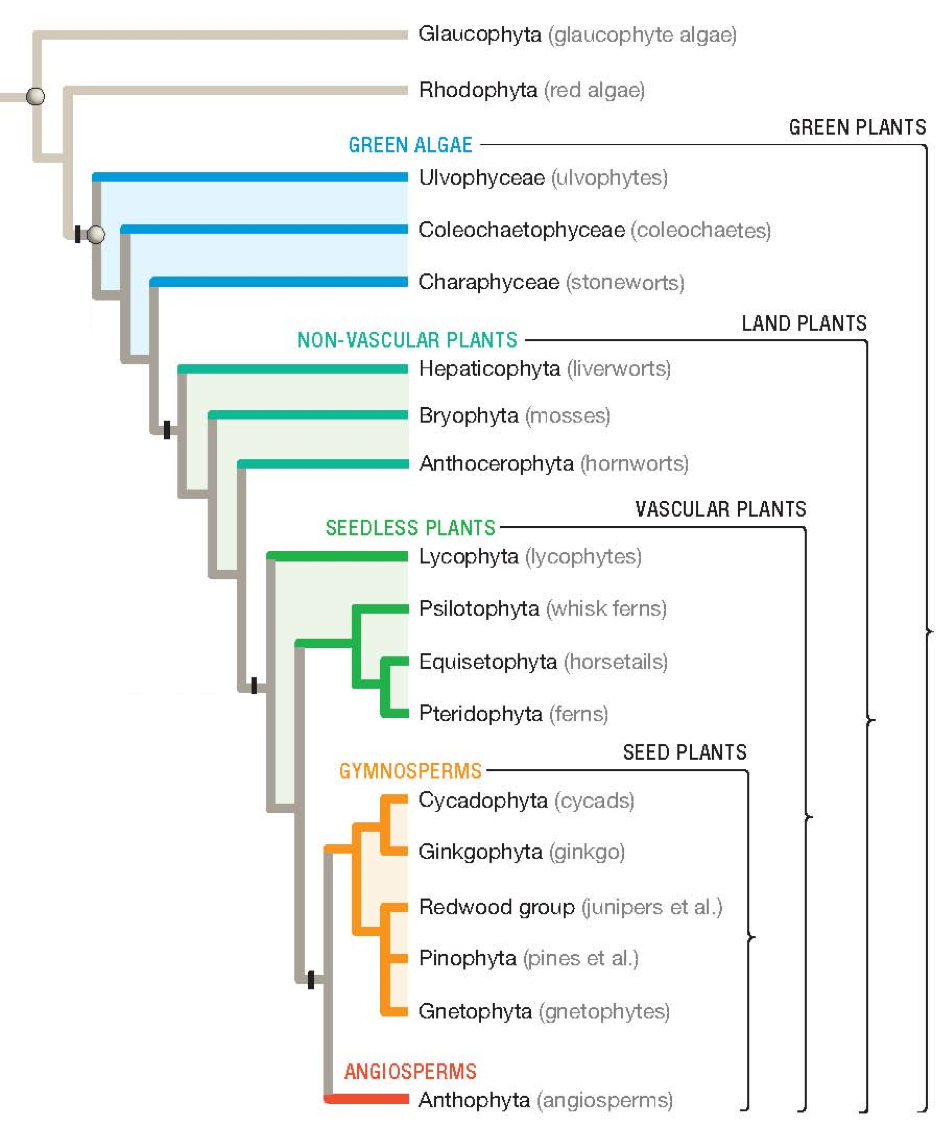
\includegraphics[height=\textheight]{plant-phylogeny.png}

        \end{columns}
    \end{adjustwidth}
    \note[item]{ID green algae: spores/zygotes (reproductive cells) with
        tough sporopollenin. Also chlorophyll types.}
    \note[item]{ID colonization of land and land plants}
\end{frame}
}

\begin{frame}
    \begin{adjustwidth}{-2em}{-1.5em}
        \begin{columns}
            \column{0.39\linewidth}

            Are the following groups monophyletic?

            \begin{itemize}
                \item Non-vascular plants

                    \nbox{No}

                \item Seedless vascular plants

                    \nbox{No}

                \item Vascular plants

                    \nbox{Yes}

                \item Seed plants

                    \nbox{Yes}

                \item Gymnosperms

                    \nbox{Yes}
            \end{itemize}

            \column{0.6\linewidth}

            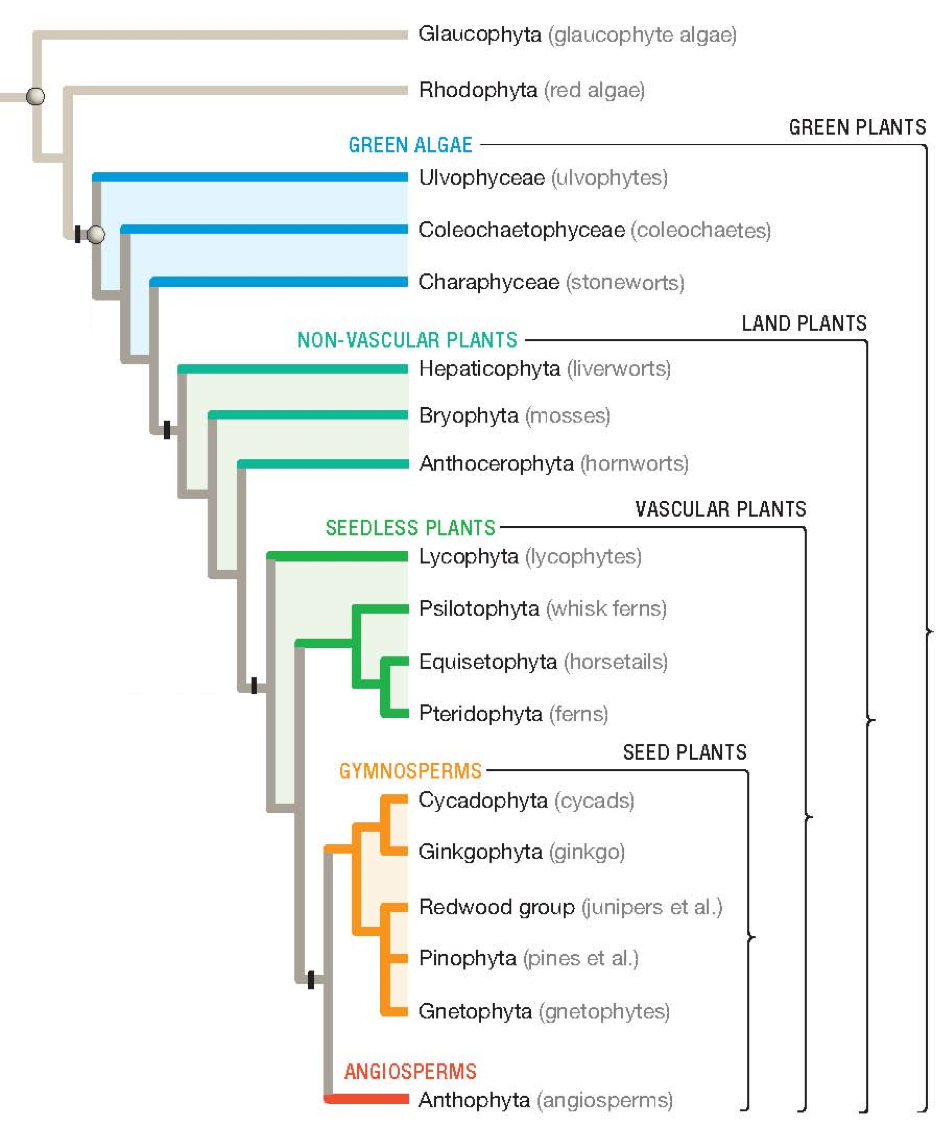
\includegraphics[height=\textheight]{plant-phylogeny.png}

        \end{columns}
    \end{adjustwidth}
\end{frame}

\clickerslide{
\begin{frame}
    \begin{clickerquestion}
        \item ``Pondweeds'' in the Charales are the sister-group (closest
            living relative) to land plants. They live in freshwater.
            
            \vspace{2mm}
            What does this suggest about the water-to-land transition in plants? 

        \begin{clickeroptions}
            \item Nothing
            \item It occurred more than once.
            \item It occurred in marine environments (where the vast majority
                of algae live today).
            \item \clickeranswer{It occurred in freshwater.}
        \end{clickeroptions}
    \end{clickerquestion}
\end{frame}
}

\begin{frame}
    \begin{adjustwidth}{-2em}{-1.5em}

        \vspace{-3mm}
        \begin{columns}
        
        \column{0.45\linewidth}

        {\small
            How big are today's liverworts, mosses, and hornworts, and what
            types of habitats do they occupy?

                \nbox{Small and primarily in wet habitats}

                \vspace{4mm}
            How big are today's gymnosperms and angiosperms, and what types of
            habitats do they occupy?

                \nbox{Large, and range from wet to dry habitats}

                \vspace{4mm}
            What do these observations suggest about trends in land plant
            evolution?

                \nbox{Increased size and ability to grow and reproduce in dry
                    areas (also a trend in the nature of the life cycle, but
                    that will be covered in BIO 220).}
        }

        \column{0.54\linewidth}

        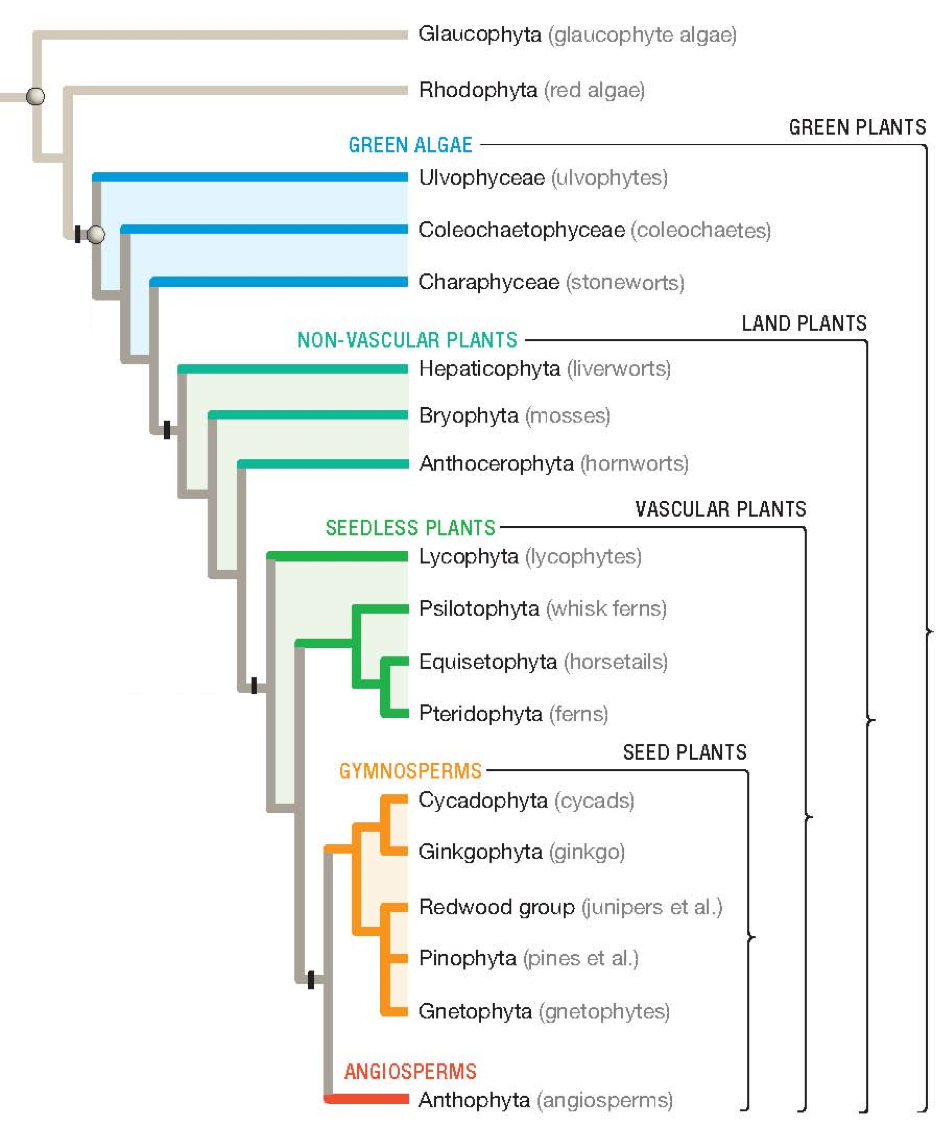
\includegraphics[width=\columnwidth]{plant-phylogeny.png}

        \end{columns}
    \end{adjustwidth}
\end{frame}

\section[Adaptation and diversification of land plants]{What adaptations
    allowed plants to colonize land and diversify?}

\clickerslide{
\begin{frame}
    \begin{clickerquestion}
        \item Given the benefits and challenges of life on land, which
            of the following is NOT true.
            
        \begin{clickeroptions}
            \item Land plants must be able to avoid desiccation (drying out).
            \item Transporting water throughout a plant's tissues is easier
                in water than on land.
            \item \clickeranswer{It is easier for plants to remain upright
                    on land than in water.}
            \item Sunlight and CO\sub{2} are more limited in water than on
                land.
            \item Transportation of gametes is more difficult on land than in
                water.
        \end{clickeroptions}
    \end{clickerquestion}
\end{frame}
}

\subsection{Living on land: cuticle, stomata, and vascular tissue}

\begin{frame}[t]
    \begin{adjustwidth}{-2em}{-1.5em}
        \vspace{-3mm}
        What adaptations allowed plants to colonize land and diversify?

        \begin{columns}[t]

        \column{0.5\linewidth}

        \begin{enumerate}
            \item Ability to avoid desiccation
            
            \begin{enumerate}
                \item<2-> Cuticle
            \end{enumerate}
        \end{enumerate}

        \vspace{-2mm}
        \uncover<2->{
        \begin{itemize}
            \small
            \item What is a cuticle?

                \nbox{Wax covering on surface (epidermal cells)}

                \vspace{6mm}
            \item Mark its origin on the tree

                \nbox{\scriptsize All land plants have cuticle---mark its
                    origin along branch of the common ancestor of all land
                    plants}

                % \vspace{1mm}
            \item What is its adaptive significance?

                \nbox{Prevents water loss from tissues}
        \end{itemize}
        }

        \column{0.5\linewidth}

            \uncover<2->{
            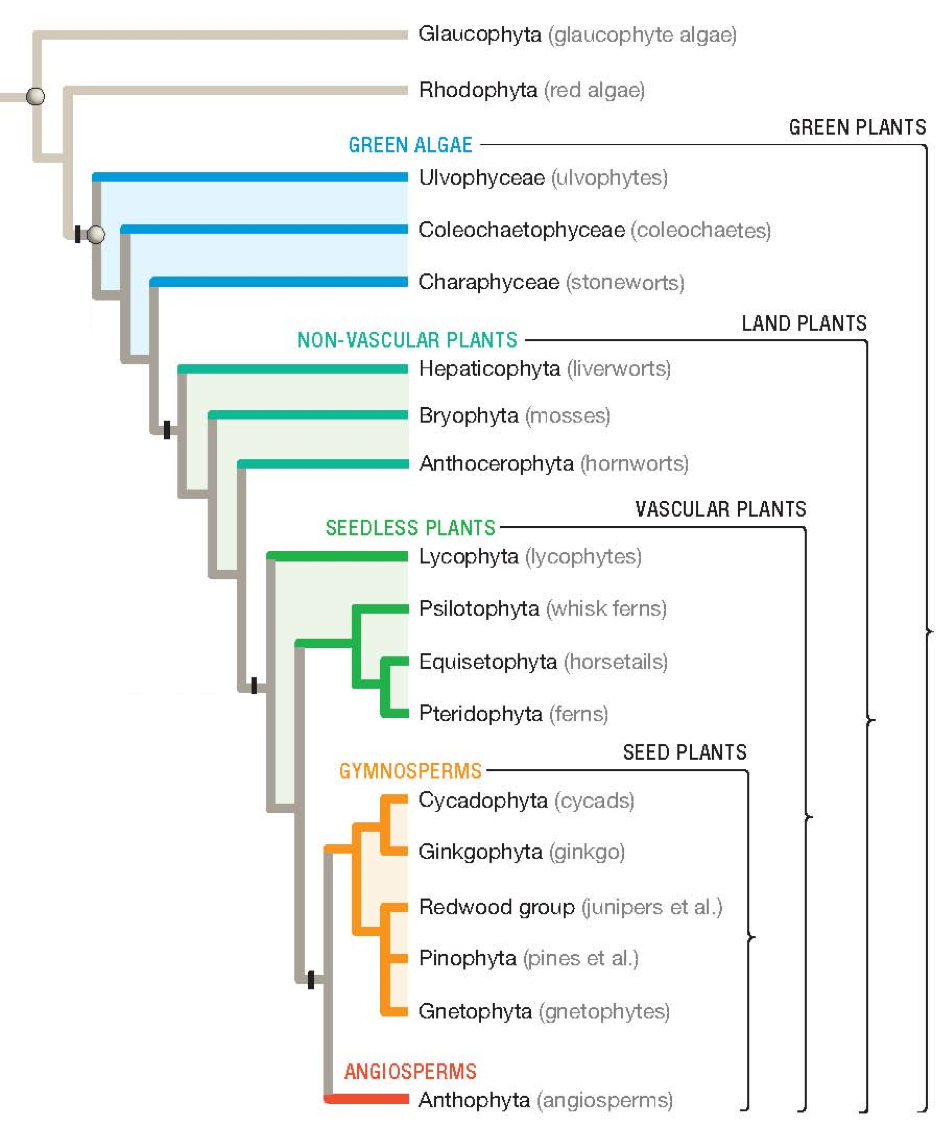
\includegraphics[width=\columnwidth]{plant-phylogeny.png}
            }

        \end{columns}
    \end{adjustwidth}
\end{frame}

\clickerslide{
\begin{frame}
    \begin{clickerquestion}
        \item The thickness of the cuticle varies widely among species. Which
            are expected to have the thickest cuticle? 

        \begin{clickeroptions}
            \item Species that lack pores or stomata. 
            \item \clickeranswer{Species that are adapted to extremely dry
                    habitats.}
            \item The bottoms of leaves. 
            \item Species in lineages that appeared recently (more derived
                groups).
            \item Species in lineages that have retained traits present in the
                earliest land plants. 
        \end{clickeroptions}
    \end{clickerquestion}
\end{frame}
}

\begin{frame}[t]
    \begin{adjustwidth}{-2em}{-1.5em}

        \vspace{-3mm}
        \begin{enumerate}
            \item Ability to avoid desiccation
            \begin{enumerate}
                \addtocounter{enumii}{1}
                \item Pores and stomata

                    \vspace{2mm}
                    Pores are found in liverworts; all other land plants have
                    stomata.

                    \uncover<2->{
                    \vspace{2mm}
                    Photosynthesis: $n \,\textrm{CO}_2 + n \,\textrm{H}_2\textrm{O} + \textrm{photons} \rightarrow (\textrm{CH}_2\textrm{O})_n + n \,\textrm{O}_2$
                    }
            \end{enumerate}
        \end{enumerate}

        \begin{columns}[t]

        \column{0.49\linewidth}

        \uncover<3->{
        \vspace{-4mm}
        \begin{itemize}
                \small
            \item What are pores? What are stomata?

                \nbox{\scriptsize Openings in the epidermis that allow gas
                    exchange.  A stoma can open/close via guard cells, whereas
                    pores cannot.}

            \vspace{2mm}
            \item Map their origin on the tree.

                \nbox{\tiny Mark origin of pore along branch of the common
                    ancestor of all land plants; mark stomata along branch of
                    ancestor leading to all land plants other than liverworts.}

            \item What is the adaptive significance of pores and stomata?

                \nbox{\scriptsize Cuticle seals off gas exchange that is
                    required for photosynthesis. Pores/cuticles allow this gas
                    exchange}

        \end{itemize}
        }

        \column{0.5\linewidth}

            \uncover<3->{
            \vspace{-4mm}
            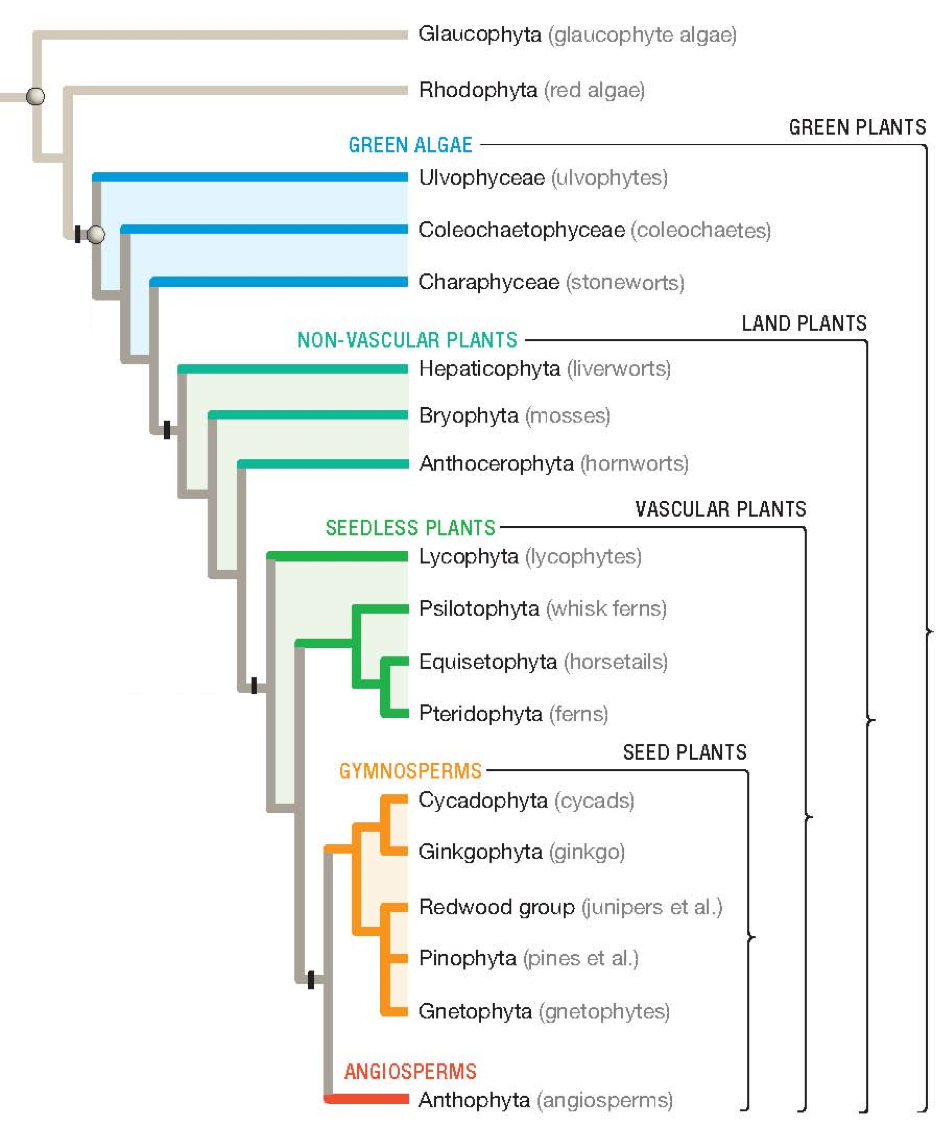
\includegraphics[width=0.9\columnwidth]{plant-phylogeny.png}
            }

        \end{columns}
    \end{adjustwidth}
\end{frame}


\begin{frame}[t]
    \begin{adjustwidth}{-2em}{-1.5em}

        \vspace{-3mm}
        \begin{enumerate}
            \addtocounter{enumi}{1}
            \item Transporting water and nutrients
            \begin{enumerate}
                \item Vascular tissue consisting of tracheids or tracheids +
                    vessels
            \end{enumerate}
        \end{enumerate}

        \begin{columns}[t]

        \column{0.49\linewidth}

        \uncover<2->{
        \vspace{-4mm}
        \begin{itemize}
            \small
            \item What is vascular tissue?

                \nbox{Groups of cells that are specialized for
                    transport of fluids}


            \vspace{4mm}
            \item Map their origin on the tree.

                \nbox{\tiny Tracheids: Along the branch of common ancestor of
                    all vascular plants. Vessels: Evolved twice independently
                    along branch leading to Angiosperms and along branch
                    leading to Gnetophytes.}

            \vspace{4mm}
            \item What is the adaptive significance of vascular tissue?

                \nbox{\scriptsize 1. Replace water lost when stomata are open.
                    2.  Transport nutrients. 3.  Structural support---cell
                    walls of water-conducting cells contain lignin.}

        \end{itemize}
        }

        \column{0.5\linewidth}

            \uncover<2->{
            \vspace{-2mm}
            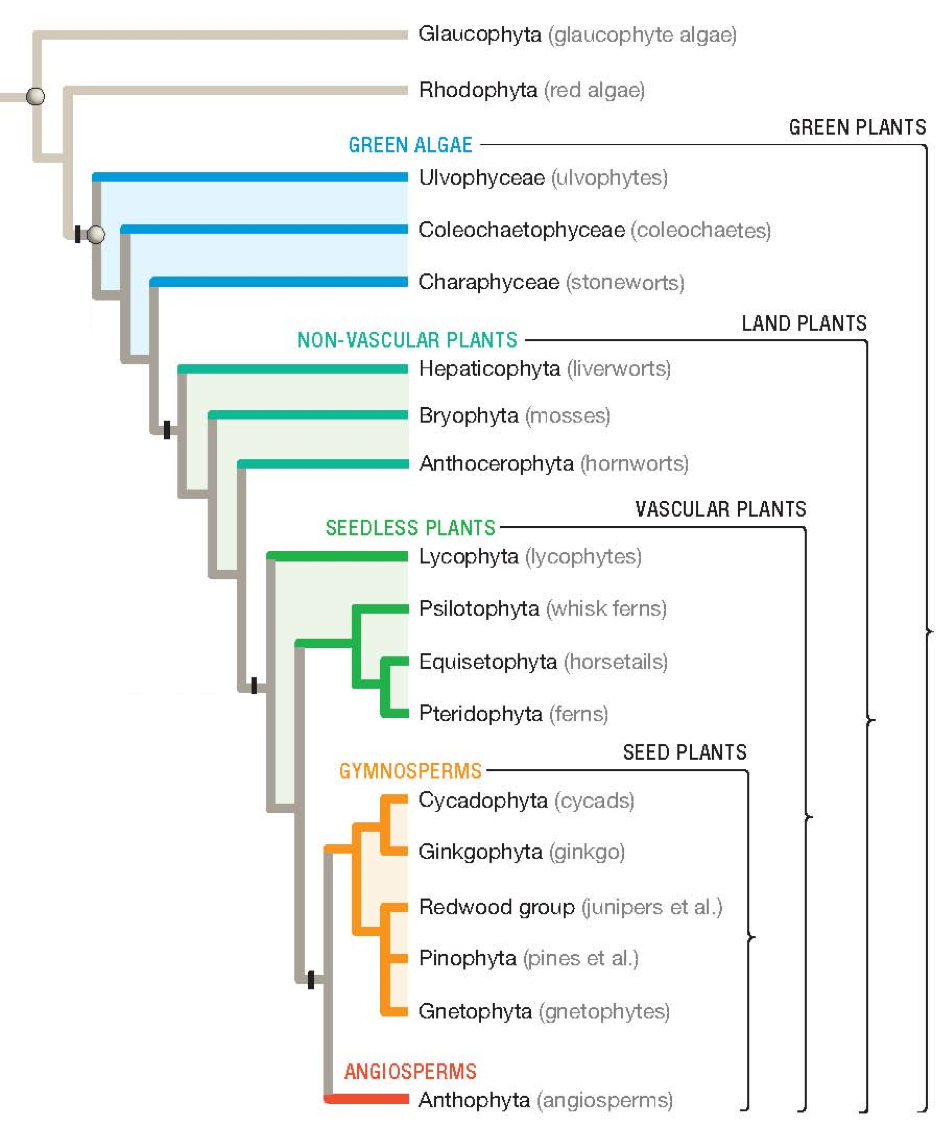
\includegraphics[width=1.0\columnwidth]{plant-phylogeny.png}
            }

        \end{columns}
    \end{adjustwidth}
\end{frame}

\subsection{Reproducing on land: embryophyte condition, pollen, and seeds}

\begin{frame}[t]
    \begin{adjustwidth}{-2em}{-1.5em}

        \begin{enumerate}
            \addtocounter{enumi}{2}
            \item The embryophyte condition
            \begin{enumerate}
                \item Gametangia are structures that enclose gamete-producing
                    cells. 

                    \uncover<2->{
                    \vspace{2mm}
                    In land plants, the egg is retained on the parent and the
                    embryo develops inside the gametangium (instead of
                    releasing zygotes).
                    }

                \uncover<3->{
                \begin{itemize}
                    \item What is the adaptive significance of the embryophyte
                        condition?

                        \nbox{Embryo receives nutrients from mom via transfer
                            cells. Embryo also is protected.}

                \end{itemize}
                }
            \end{enumerate}
        \end{enumerate}
    \end{adjustwidth}
\end{frame}

\clickerslide{
\begin{frame}
    \begin{clickerquestion}
        \item Which of the following mammalian structures or events performs a
            function analogous to that of the transfer cells in embryophytes?  
 
        \begin{clickeroptions}
            \item \clickeranswer{Placenta}
            \item Paternal care (feeding of offspring by male parent)
            \item Lactation (milk production and nursing)
            \item Womb (uterus)
        \end{clickeroptions}
    \end{clickerquestion}
\end{frame}
}


\begin{frame}[t]
    \begin{adjustwidth}{-2em}{-1.5em}

        \begin{enumerate}
            \addtocounter{enumi}{3}
            \item Pollen
            \begin{enumerate}
                \item Cells that are encased in tough coat of sporopollenin;
                    some give rise to sperm cells.

                    \uncover<2->{
                    \vspace{2mm}
                    Transported from one plant to another by wind, animals, or
                    water.
                    }

                \uncover<3->{
                \begin{itemize}
                    \item What is the adaptive significance of pollen?  (HINT:
                        In ferns, mosses, and other plants that lack pollen,
                        sperm have to swim to the egg.)
                        % and/or hitch a ride on
                        % legs of tiny insects.)

                        \nbox{Sperm are protected from desiccating (drying
                            out)---can travel longer distances to fertilize and
                            have higher reproductive success.}

                \end{itemize}
                }
            \end{enumerate}
        \end{enumerate}
    \end{adjustwidth}
\end{frame}


\begin{frame}[t]
    \begin{adjustwidth}{-2em}{-1.5em}

        \begin{enumerate}
            \addtocounter{enumi}{4}
            \item The seed
            \begin{enumerate}
                \item An embryo with a food supply, surrounded by a tough coat.

                    \vspace{2mm}
                    Transported away from the parent by wind, animals, or
                    water.

                \uncover<2->{
                \begin{itemize}
                    \item What is the adaptive significance of the seed?
                        (HINT: In ferns, mosses, and other plants that lack
                        seeds, the dispersal stage is a single-celled spore.)

                        \nbox{Offspring grow away from parent---less
                            competition with parents. Embryo protected and gets
                            nutrients from mom, which gives seedlings a head
                            start.}

                \end{itemize}
                }
            \end{enumerate}
        \end{enumerate}
    \end{adjustwidth}
\end{frame}

\end{document}

\clickerslide{
\begin{frame}
    \begin{clickerquestion}
        \item 
        \begin{clickeroptions}
            \item 
            \item 
            \item 
            \item 
        \end{clickeroptions}
    \end{clickerquestion}
\end{frame}
}

\clickerpost{
{
\usebackgroundtemplate{\includegraphics[page=17,width=\paperwidth]{./24-Radiation-extinction.pdf}}
\begin{frame}[t,plain]
    \begin{adjustwidth}{-2em}{-1.5em}
        \cmask{Answer: 3}
    \end{adjustwidth}
\end{frame}
}
}

